\documentclass[12pt]{article}
\usepackage{titlesec}
\usepackage{bm}
\usepackage{amsmath}
\usepackage{amsfonts}
\usepackage{amssymb}
\usepackage{graphicx}
\usepackage{colortbl}
\usepackage{xr}
\usepackage{hyperref}
\usepackage{longtable}
\usepackage{xfrac}
\usepackage{tabularx}
\usepackage{float}
\usepackage{soul}
\usepackage{siunitx}
\usepackage{booktabs}
\usepackage{array}
\usepackage{graphicx}
\newcolumntype{C}[1]{>{\centering\let\newline\\\arraybackslash\hspace{0pt}}m{#1}}
\graphicspath{ {images/} }

\hypersetup{
    bookmarks=true,         % show bookmarks bar?
      colorlinks=true,       % false: boxed links; true: colored links
    linkcolor=black,          % color of internal links (change box color with linkbordercolor)
    citecolor=green,        % color of links to bibliography
    filecolor=magenta,      % color of file links
    urlcolor=cyan           % color of external links
}
\newcommand{\wss}[1]{\authornote{magenta}{SS}{#1}}
\newcommand{\hed}[1]{\authornote{blue}{HM}{#1}} %Hediyeh
\newcommand{\tz}[1]{\authornote{blue}{TZ}{#1}} %Tahereh
\newcommand{\pl}[1]{\authornote{blue}{PL}{#1}} %Peng

\newcommand{\colZwidth}{1.0\textwidth}
\newcommand{\blt}{- } %used for bullets in a list
\newcommand{\colAwidth}{0.13\textwidth}
\newcommand{\colBwidth}{0.82\textwidth}
\newcommand{\colCwidth}{0.1\textwidth}
\newcommand{\colDwidth}{0.05\textwidth}
\newcommand{\colEwidth}{0.8\textwidth}
\newcommand{\colFwidth}{0.17\textwidth}
\newcommand{\colGwidth}{0.5\textwidth}
\newcommand{\colHwidth}{0.28\textwidth}
\newcounter{defnum} %Definition Number
\newcommand{\dthedefnum}{GD\thedefnum}
\newcommand{\dref}[1]{GD\ref{#1}}
\newcounter{datadefnum} %Datadefinition Number
\newcommand{\ddthedatadefnum}{DD\thedatadefnum}
\newcommand{\ddref}[1]{DD\ref{#1}}
\newcounter{instnum} %Instance Number
\newcommand{\itheinstnum}{IM\theinstnum}
\newcommand{\iref}[1]{IM\ref{#1}}
\newcounter{reqnum} %Requirement Number
\newcommand{\rthereqnum}{P\thereqnum}
\newcommand{\rref}[1]{R\ref{#1}}
\newcounter{lcnum} %Likely change number
\newcommand{\lthelcnum}{LC\thelcnum}
\newcommand{\lcref}[1]{LC\ref{#1}}

\newcommand{\tclad}{T_\text{CL}}
\newcommand{\degree}{\ensuremath{^\circ}}
\newcommand{\progname}{SWHS}

\usepackage{fullpage}

\begin{document}

\begin{titlepage}
\font\myfont=cmr12 at 38pt
\title{\myfont\vspace{60mm}Zop Test Plan} 
\author{Ratna Emani, Cole Blanchard, Akshay Mantha}
\date{\today}
\maketitle

\end{titlepage}

\newpage
\textbf{Revision History}\\
\begin{center}
 \begin{tabular}{|C{3cm}|C{3cm}|C{3cm}|C{3cm}|}
 \hline
 \textbf{Developer} & \textbf{Date} & \textbf{Change} & \textbf{Revision Number}\\
 \hline \hline
 \textcolor{red}{Akshay Mantha} & \textcolor{red}{December 7 2015} & \textcolor{red}{Testing Schedule (Akshay)}  & 9\\
 \hline
 \textcolor{red}{Cole Blanchard} & \textcolor{red}{December 7 2015} & \textcolor{red}{Performance Testing}  & 8\\
 \hline
 \textcolor{red}{Ratna Emani} & \textcolor{red}{December 7 2015} & \textcolor{red}{Testing Schedule (Ratna), \newline Usability Testing} & 7\\
 \hline
 Ratna Emani & November 27 2015 & Update Tex file & 6\\
 \hline
 Akshay Mantha & November 27 2015 & Update Test plan & 5\\
 \hline
 Cole Blanchard & October 23 2015 & 3.5 Board Update Test, \newline 3.6 Tile Adjacency Check & 4\\
 \hline
 Ratna Emani & October 23 2015 & Reliability,\newline Maintainability, \newline Correctness, Ease of Use,\newline 3.4 Raw Game-play Test & 3\\
 \hline
 Akshay Mantha & October 22 2015 & 3.1(...)Score Are the Same,\newline 3.2(...)Score Are Not the Same, \newline 3.3 Match of Tiles & 2\\
 \hline
 Ratna Emani & October 22 2015 & File Development, \newline Formatting & 1\\
 \hline
 \end{tabular}
\end{center}

\newpage
\tableofcontents
\newpage


%%%%%%%%%%%%%%%%%%%%%%%%
%
%	1.) General Information 
%
%%%%%%%%%%%%%%%%%%%%%%%%

\section{Introduction}


%1.1 Reliability 
\subsection{Reliability}
Reliability takes precedence over efficiency. It often relies on and involves the redundant checking for exceptional conditions within the program. Many developers often show negligence when testing for reliability. There is a lack of defined depth which programmers deem exceptional conditions necessary, often risking reliability in the process. Given an error it is of the utmost importance that the application must respond appropriately. Errors include values passed by users that are out of the input domain range, warnings that direct users for any potential unwanted behaviours is stimulated by the program. These can be controlled my managing the user accessibility to sensitive values that may cause problems to the internal functions of the program.  Also, by keeping the user’s input domain to a minimum, the program has less possibility to run into errors. 

%1.2 Maintainability 
\subsection{Maintainability}
Software maintainability is the foothold of a successful program. Maintainability is great tool shared amongst developers that allow the application to expand and adopt. With an open-source project like this, it is crucial to keep the program well maintained, allowing other developers to implement furthermore. The lack for maintainability is the main cause for the demise of a program. Once this program has been made by our development team, it will be back up as an open-source project. Support and maintenance will be provided by other developers that will use the game to expand or evolve to new measures.\\\\
The game has to potential to change in many different ways. From the addition of new controls, to reinventing the game rules, the possibilities can be endless. As a development team, we chose to use modularity to increase maintainability of the program. By making the application more object-oriented it allows other developers to easily understand and apply their changes with minimum effort. With the use of simple modules and strong internal cohesion the program will maximize the performance as well.



%1.3  Correctness
\subsection{Correctness}
Test cases allows the development team and the client to test the final product for correctness. Correctness is a degree to which a program’s behaviour matches its requirements, essentially a tool to measure quality and robustness. It is important for the development team to deliver what was promised in the specifications. However, it is crucial for the program to be error free, to keep the user engaged at all times. The lack of free flow in game design or bugs can easily put off players. Therefore it is crucial that the game does not diverging from a specification and updates its rules to maintain correctness. 


%1.4 Ease of Use
\subsection{Ease of Use}
Ease of use defines the extent to which the program can be used to achieve the results required by the user. Setting a low barrier of entry shuns the users away from feeling conformable with the application. This means that the user interface must be simple and minimal in structure. The program must be accurate and fast, in which the users can play the game and get the results they expect, efficiently. 
One way to make this possible is to minimize the user input to simple (straightforward) instructions. The game itself uses the clicker input from a frame of the game's interface. Furthermore, the game separates its shell buttons from the actual core gaming, to avoid any accidental disruption during the gaming session.  This allows the game to be more engaging and satisfying to use.  

%%%%%%%%%%%%%%%%%%%%%%%%
%
%	2.) Automation Plans
%
%%%%%%%%%%%%%%%%%%%%%%%%

\section{Automation Plans}
Automated PyUnit testing will be used to ensure that the internal functions are operating correctly. Each function and objects will be tested by passing the appropriate values from the input domain range including the extremes. Some of the places automated testing can be used for is checking of the score board, checking if the colors of the selected tiles are matching correctly and if the tiles being generated are all within the color range. \st{White box testing or Structural testing will not be automated for this program}. We would like to use automation to mainly check functionality of the application. 
\textcolor{red}{\subsection{Unit Testing}
We will make use of the 'unittest' (of Python). We do not need drivers, but we will be using stubs for most of the unit tests. Stubs, mostly, include creating instances and objects of the involved (in testing a specific method) methods.
As for code coverage metrics, we did not quantify the coverage, but we tested (covered) all important methods from all modules.}

\newpage
%%%%%%%%%%%%%%%%%%%%%%%%
%
%	3.) System Tests
%
%%%%%%%%%%%%%%%%%%%%%%%%

\section{System Tests}
\textcolor{red}{Systems tests will, primarily, utilise the Logic.py module, which in turn utilises the Board.py module (which itself utilises the Tile.py module). This is a way in that the existing implementation will be tested.}
%3.1 Tile(s) Removed and Value is set to 0
\subsection{Tile(s) Removed and Value is set to 0}
\subsubsection{Test type}
Automated, unit test
\subsubsection{Initial state}
The board is initialized, size of 6 by 6; 36 blocks in place.
\subsubsection{Input}
Tile(s) removed (after matching).
\subsubsection{Output}
The value of tile(s) removed is 0.
\subsubsection{Schedule}
This feature will be implemented for the Proof of Concept Demonstration.
\subsubsection{Methodology}
This test can be done using PyUnit (unit-testing framework) in PyCharm (an IDE). PyUnit should pass the test case.
\subsubsection{Test tool}
Integration testing can be used as a tool to see how this function communicates with other functions of the system.
\subsubsection{Test for}
This test validates the "happy path" scenario of updated score requirement. 

\newpage

%3.2 Tile(s) Removed and Value is not set to 0
\subsection{Tile(s) Removed and Value is not set to 0}
\subsubsection{Test type}
Automated, unit test
\subsubsection{Initial state}
The board is initialized, size of 6 by 6; 36 blocks in place.
\subsubsection{Input}
Tile(s) removed (after matching).
\subsubsection{Output}
The value of tile(s) removed is not 0.
\subsubsection{Schedule}
This feature will be implemented for the Proof of Concept Demonstration.
\subsubsection{Methodology}
This test can be done using PyUnit (unit-testing framework) in PyCharm (an IDE). PyUnit should pass the test case.
\subsubsection{Test tool}
Integration testing can be used as a tool to see how this function communicates with other functions of the system.
\subsubsection{Test for}
This test validates the negative scenario of  removing tile (leads to unupdated score) requirement. 

\newpage

%3.3 Colour Match of Blocks
\subsection{Colour Match of Tiles}
\subsubsection{Test type}
Automated, unit test
\subsubsection{Initial state}
The board is initialized, size of 6 by 6; 36 tiles in place.
\subsubsection{Input}
Coordinates of tiles are given to the function.
\subsubsection{Output}
A Boolean value; true when the selected tiles' colour is the same.
\subsubsection{Schedule}
This feature will be implemented for the Proof of Concept Demonstration.
\subsubsection{Methodology}
This test can be done automatically using PyUnit. The tester will give PyUnit the funciton. Then, PyUnit should execute the test and pass it.
\subsubsection{Test tool}
Unit testing framework can be used as a tool to see how this function works within the scope of the system. 
\subsubsection{Test for}
This test validates the requirement of selecting tiles of same colour to obtain a score.

\newpage

%3.4 Board Update Test
\subsection{Board Update Test}
\subsubsection{Test type}
Automated, Structural test
\subsubsection{Initial state}
State after removing tiles from the board (some spaces are empty).
\subsubsection{Input}
6x6 array (empty spaces flagged).
\subsubsection{Output}
6x6 array (no empty spaces remaining, tiles above move down to fill empty spaces).
\subsubsection{Schedule}
This feature will be implemented for the Proof of Concept Demonstration.
\subsubsection{Methodology}
Using PyUnit, the test will remove 0-6 blocks in a column. PyUnit should execute and ensure the tiles above move into the correct space in the next state of the board. Then it will ensure there are no more empty spaces on the board. 
\subsubsection{Test tool}
Unit testing can be used to see how the function works within the system.
\subsubsection{Test for}
The test validates that all empty spaces in the previous state of the board have been filled with the tiles above it in the next state as well as randomly coloured blocks to fill in spaces which do not have tiles above.

\newpage

%3.5 Tile Adjacency Check
\subsection{Tile Adjacency Check}
\subsubsection{Test type}
Automated, unit test
\subsubsection{Initial state}
Board is initialized, 6x6 array. 
\subsubsection{Input}
Coordinates of blocks are given
\subsubsection{Output}
Boolean value is given; True when blocks are directly next to each other, False otherwise.
\subsubsection{Schedule}
This feature will be implemented for the Proof of Concept Demonstration.
\subsubsection{Methodology}
Using PyUnit, the test will ensure that any tiles selected by the user are next to each other, in one direct path (i.e. no overlapping).
\subsubsection{Test tool}
Unit testing can be used to see how the function works in the system.
\subsubsection{Test for}
The test validates that tiles being removed are next to each other, in a direct path (horizontal or vertical only).

\newpage

%3.6 Type Exception Check (While Moving Tiles Down)
\subsection{Type Exception Check (While Moving Tiles Down)}
\subsubsection{Test type}
Automated, Structural test
\subsubsection{Initial state}
Board is initialized; 6x6 array.
\subsubsection{Input}
Column number, instance of boad, and an integer representing the number of empty spaces (in a column). 
\subsubsection{Output}
Assertion should throw a 'TypeError' if either the column number is not an integer, some other object/class is instantiated instead of board, and there is no integer to represent the number of empty spaces (in a column).
\subsubsection{Schedule}
This feature will be implemented for the Final Presentation.
\subsubsection{Methodology}
PyUnit will see, if parameters of the moveDown method are of correct type or not. 
\subsubsection{Test tool}
Unit testing can be used to see how robust the function is with respect to parameters.
\subsubsection{Test for}
The test validates throwing exceptions.

\textcolor{red}{\section{Non Functional Testing}
\subsection{Usablity Testing}
Usability testing is a proficient way of measure real-user experience of any application. Companies that launch an software products usually dedicate a team of users called a focus group to test this. Followed by Alpha, and Beta testing done by select users/consumers. For usablility testing of Zop, we decided to ask few friends to play the game and write their suggestions/concerns as feedback.
\subsection{Performance Testing}
Performance testing is a good way of seeing how efficient the program it running.  It measures the speed of functions and how many times they are called throughout the program.  In Zop, performance testing will be measured by how many times functions are called throughout the program.  This will accomplish seeing how we can make the program better for the final product.}

\textcolor{red}{\section{Test Scheduling}
\begin{table}[h!]
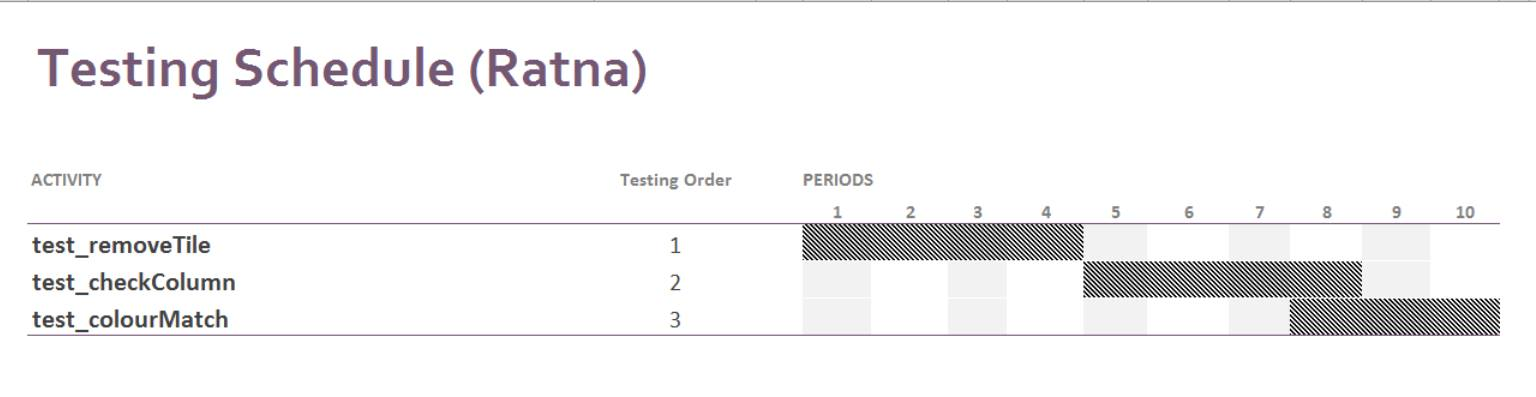
\includegraphics[width = 17cm]{ratnaSchedule}
\caption{Testing Schedule 1}
\end{table}
\begin{table}[h!]
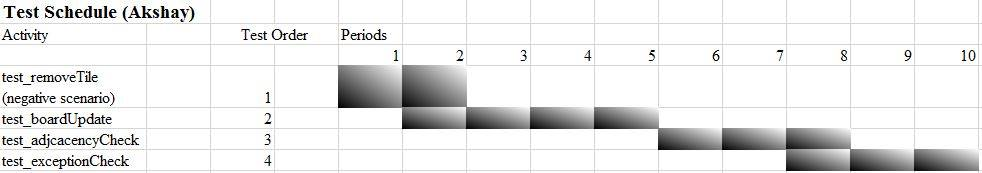
\includegraphics[width = 17cm]{akshaySchedule}
\caption{Testing Schedule 2}
\end{table}}


\end{document}